\section{The PDE and the learning tasks}
\label{sec:math}
\subsection{What NLS describes}
An envelope describes the slowly varying amplitude and phase of an
oscillatory wave. For example, a leading-order surface signal has the form
\[
 \eta(x,t)\approx\Repart\{B(x,t)e^{\ii(k_0x-\omega_0t)}\}.
\]
The complex field $B$ contains information about both the height and the
position of the carrier oscillations. Matching $|B|$ alone therefore does
not ensure accurate surface-wave prediction. Envelope-to-surface conversion,
including any retained bound harmonics, must be specified consistently.

A common mathematical normalization of cubic NLS is
\begin{equation}
 \ii q_s+p q_{yy}+\gamma |q|^2q=0,
 \qquad (s,y)\in[0,S]\times\mathbb T_L,
 \label{eq:nls}
\end{equation}
where $q$ is complex, $s$ is an evolution variable, $y$ is a profile
coordinate, $p,\gamma\in\RR$, and $\mathbb T_L=\RR/(L\mathbb Z)$.
Dispersion is represented by $p q_{yy}$ and nonlinear phase modulation by
$\gamma|q|^2q$. Under this convention $p\gamma>0$ is the focusing case;
$p\gamma<0$ is the defocusing case. Signs and scalings vary across papers.
An equation written in laboratory time is not automatically the same
experimental problem as spatial propagation of a retarded-time envelope.

Bright solitons, dark solitons on a background, breathers, and rogue-wave
profiles supply useful test cases. They should not substitute for testing
general random packets, interactions, changed initial conditions, or noisy
observations. Higher-order, variable-coefficient, coupled, and nonlocal NLS
models introduce further terms and may have different invariants and
well-posedness assumptions.

For smooth periodic solutions of \eqref{eq:nls}, standard conserved
quantities are mass (or action), momentum, and Hamiltonian:
\begin{align}
 M[q]&=\int_{\mathbb T_L}|q|^2\dd y,&
 P[q]&=\Impart\int_{\mathbb T_L}\overline q q_y\dd y,\notag\\
 H[q]&=\int_{\mathbb T_L}
       \left(p|q_y|^2-\frac{\gamma}{2}|q|^4\right)\dd y.
 \label{eq:nlsinvariants}
\end{align}
These expressions assume the stated normalization and boundary conditions.
On the real line, their use also requires suitable integrability. They are
not a license to impose the same constraints on a different envelope model.

\subsection{How a PINN is used}
A conventional PINN represents $q_\theta=a_\theta+\ii b_\theta$ by two real
network outputs. Its NLS residual has real and imaginary parts
\begin{align*}
 r_a&=-\partial_s b_\theta+p\partial_{yy}a_\theta
          +\gamma(a_\theta^2+b_\theta^2)a_\theta,\\
 r_b&=\partial_s a_\theta+p\partial_{yy}b_\theta
          +\gamma(a_\theta^2+b_\theta^2)b_\theta.
\end{align*}
Automatic differentiation supplies the local derivatives. Complex-valued
networks instead use complex internal parameters or operations; both
representations can express a complex solution. Their relative usefulness
is an empirical question about trainability and inductive bias.

A representative objective is
\begin{equation}
 \mathcal L=\lambda_r\sum_j w_j|r_\theta(z_j)|^2
  +\lambda_0\mathcal L_0+\lambda_b\mathcal L_b
  +\lambda_d\mathcal L_d+\lambda_I\mathcal L_I.
 \label{eq:loss}
\end{equation}
Here $z_j=(s_j,y_j)$ are residual points; $\mathcal L_0$ and
$\mathcal L_b$ measure initial and boundary errors;
$\mathcal L_d$ compares an observation operator applied to $q_\theta$
with data; and $\mathcal L_I$ optionally measures invariant defects.
Weights require scaling and validation. A small value of this sampled,
weighted objective is not itself a bound on the solution error. This basic
framework has a direct NLS precedent in Raissi et al. \cite{raissi}.

\begin{longtable}{@{}P{0.17\textwidth}P{0.35\textwidth}P{0.40\textwidth}@{}}
\toprule
Task & What is learned & Appropriate test \\
\midrule
Forward solve & A field for one specified initial condition and PDE. &
Error and total solve time against a converged numerical solution. \\
Inverse problem & Coefficients, latent initial field, or both, from observations. &
Identifiability, noisy-data robustness, and withheld observations. \\
Assimilation & A consistent field over the observed region. &
Reconstruction at withheld locations; distinguish interpolation from forecast. \\
Operator learning & A map from initial fields or measurements to solution fields. &
Completely unseen trajectories and amortized cost including training. \\
\bottomrule
\end{longtable}
A network trained on one soliton does not become a general solution operator
because it can be evaluated at arbitrary coordinates. A PINO or
physics-informed DeepONet is trained across inputs to learn such a map
\cite{pino}. The same distinction applies to sensor-conditioned models.

\subsection{The approved water-wave Dysthe equation}
The current project contract specifies
\begin{equation}
\begin{split}
 u_\xi={}&-\ii u_{\tau\tau}-\ii|u|^2u\\
 &-\varepsilon\left(8|u|^2u_\tau
       +2u^2\overline{u_\tau}
       +2\ii u\,|D_\tau|(|u|^2)\right).
\end{split}
\label{eq:dysthe}
\end{equation}
Here $\xi$ is propagation distance, $\tau$ is retarded time, $u$ is the
scaled free-surface envelope, and $\varepsilon$ is carrier steepness in the
specified formal normalization. This convention agrees with the
free-surface equation (1.3) of Fedele--Dutykh \cite{fedele}. In the source
coordinates, $\tau=\varepsilon(2x-t)$, $\xi=\varepsilon^2x$, and
$B=\varepsilon u$. Setting $\varepsilon=0$ defines a mathematical NLS
control; the physical coordinate map is not invertible at zero steepness.

On periodic profiles, the nonlocal operator is
\[
 \widehat{|D_\tau|f}(k)=|k|\widehat f(k),
 \qquad k=2\pi n/L,\quad n\in\mathbb Z.
\]
For the forward Fourier convention $e^{-\ii k\tau}$,
$|D_\tau|=\mathcal H\partial_\tau$; its zero mode is zero. This term
depends on the full profile. Differentiating a pointwise neural output at
isolated random points does not evaluate this operator.

The free-surface field is noncanonical. Use the correct transformed
invariants and boundary convention if imposing an energy or momentum
constraint. The potential-envelope equation, whose corresponding
conjugate-derivative coefficient is zero, is a different formulation.
The shared model file also requires periodic grids without a duplicated
endpoint, complex arrays with axes $(\xi,\tau)$, and whole-initial-field
data splits. Two array axes are not two horizontal physical directions.

\section{Why a good-looking NLS solution is insufficient}
\label{sec:failure}
There are several independent sources of failure: an inappropriate PDE;
insufficient observation information; an unresolved reference calculation;
a network that does not represent the relevant oscillations; and training
that does not reach the relevant solution. Improving an optimizer only
addresses part of this chain.

For oscillatory problems, important practical issues are spectral bias,
imbalanced initial/boundary/residual gradients, large residual regions
dominating small localized events, accumulated phase error, and inconsistent
boundary conditions. Hard constraints, causal weighting, adaptive sampling,
and better curvature information address different mechanisms
\cite{hardic,causal,gravis,urban,soap}.

\begin{example}[Conservation can miss accumulated phase error]
On any periodic profile domain, consider
\[
 q(s,y)=e^{2\ii s},\qquad
 v(s,y)=e^{\ii(2+\delta)s},\qquad \delta\in\RR.
\]
The first solves \eqref{eq:nls} with $p=1$, $\gamma=2$. Both fields have
the same initial data, amplitude, mass, momentum, and Hamiltonian. Yet
\[
 r[v]=-\delta v,\qquad
 \frac{\norm{v(s)-q(s)}_{L^2}}{\norm{q(s)}_{L^2}}
       =2\abs{\sin(\delta s/2)}.
\]
Thus a small persistent residual can accumulate a large phase error.
This is an exact analytic illustration, not a trained-network result.
\end{example}

\begin{figure}[htbp]
\centering
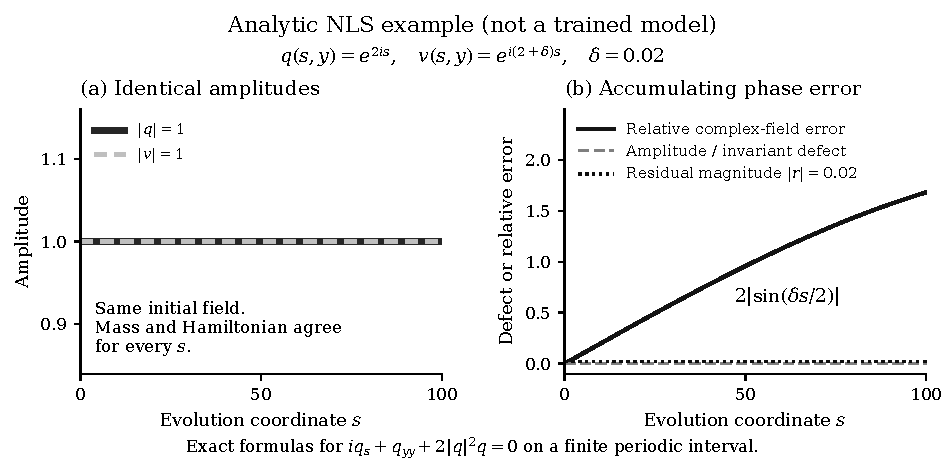
\includegraphics[width=0.95\textwidth]{figures/phase-drift.pdf}
\caption{Exact illustration with $\delta=0.02$. Amplitude and invariant
defects are zero, while complex-field error grows over the plotted interval.
The residual magnitude stays at $0.02$. No PINN or Dysthe experiment is
represented.}
\label{fig:phase}
\end{figure}

\begin{proposition}[A conditional NLS residual estimate]
Let $q,v$ be sufficiently smooth periodic fields on
$[0,S]\times\mathbb T_L$, with $q$ solving \eqref{eq:nls} and
$r=\ii v_s+p v_{yy}+\gamma|v|^2v$. Assume $p,\gamma$ are real and
$|q|,|v|\leq B$ everywhere. Then, for $0\leq s\leq S$,
\begin{equation}
 \norm{v(s)-q(s)}_2\leq e^{3|\gamma|B^2s}
 \left(\norm{v(0)-q(0)}_2+
          \int_0^s\norm{r(t)}_2\dd t\right).
 \label{eq:stability}
\end{equation}
\end{proposition}
\begin{proof}
Set $e=v-q$. The periodic linear Schr\"odinger part contributes zero
to the real $L^2$ energy derivative. The pointwise inequality
$\bigl||v|^2v-|q|^2q\bigr|\leq3B^2|v-q|$ and Cauchy--Schwarz give
$\frac{\mathrm d}{\mathrm ds}\norm e_2
\leq3|\gamma|B^2\norm e_2+\norm r_2$ wherever the norm is nonzero.
Regularization of the norm gives the same integral inequality at its
zeros. Gronwall's inequality yields \eqref{eq:stability}.
\end{proof}
This elementary estimate is included for explanation, not as a novel
theorem. It requires a continuous residual norm, initial-error control, and
amplitude bounds; a training mean-squared error does not supply these
automatically. Its exponential factor can be pessimistic. It does not prove
an analogous estimate for Dysthe's derivative and nonlocal nonlinearities.
The more refined NLS theory discussed below uses different norms and
explicit integration assumptions \cite{alejo}.
